\documentclass[11pt]{article}

\usepackage[utf8]{inputenc}
\usepackage[french]{babel}

\usepackage[a4paper,margin=1in,portrait]{geometry}

\usepackage[table]{xcolor}
\definecolor{lightgray}{gray}{0.85}
\definecolor{verylightgray}{gray}{0.95}
\let\oldtabular\tabular
\let\endoldtabular\endtabular
\renewenvironment{tabular}{\rowcolors{1}{lightgray}{verylightgray}\oldtabular}{\endoldtabular}

% Pour le bas de page
\newcommand{\mysmallgray}[1]{\scriptsize\color{gray}#1}

\usepackage{comment}

%\usepackage{multicol}
%\setlength{\columnsep}{0.5cm}
%\usepackage{wrapfig}

\usepackage{graphicx}

\usepackage{hyperref}
\hypersetup{
colorlinks=true,
linkcolor=blue,
urlcolor=blue,
}

\usepackage{fancyhdr}
\pagestyle{fancy}
\fancyhead[L]{}
\fancyhead[C]{{\color{violet}\textbf{{\Huge R}{\LARGE ISUS - }{\Huge R}{\LARGE ÈGLES POUR }{\Huge M}{\LARGE ÉGA}}}}
\fancyhead[R]{}

\fancyfoot[L]{\mysmallgray{Version 1.0}}
\fancyfoot[C]{\mysmallgray{\today}}
\fancyfoot[R]{\mysmallgray{Copyleft \href{https://github.com/orey/jdr-risus}{Olivier Rey}}}
\renewcommand{\headrulewidth}{0.4pt}
\renewcommand{\footrulewidth}{0.4pt}

% Enlève l'indentation pour tout le documnt (équivalent de \noindent sur toutes les lignes)
%\setlength\parindent{0pt}

% Sections avec points après les numéros
\usepackage{titlesec}
\titlelabel{\thetitle.\quad}
\titleformat*{\section}{\color{violet}\bfseries\Large}
\titleformat*{\subsection}{\color{violet}\bfseries\large}
\usepackage[dotinlabels]{titletoc}

%\AtBeginDocument{
%  \addtocontents{toc}{\footnotesize}
%  \addtocontents{lof}{\footnotesize}
%}

% Mes macros

\newcommand{\mysection}[1]{
\vspace{0.2cm}
\noindent{\color{violet}\large\textbf{#1}}
}

\newcommand{\mysubsection}[1]{
\vspace{0.1cm}
\noindent{\textit{\textbf{#1}}}
}


%=======================================DOC
\begin{document}

%=============== Title page

\pagestyle{empty}

\begin{center}

\includegraphics[scale=0.30]{logo-risus}

\vspace{1.0cm}


\includegraphics[scale=1.0]{logo-mega-red}

\vfill

\begin{tabular}{ll}
Méga 1            & L'origine \href{https://archive.org/details/jeux-et-strategie-hs-1}{Méga 1} \\
Méga 2            & L'indispensable \href{https://archive.org/details/jeux-et-strategie-hs-2}{Méga 2} \\
Méga 3            & Ne peut être trouvé qu'en occasion, voir la fiche \href{https://www.legrog.org/jeux/mega/mega-3/mega-iii-fr-47583}{Grog} \\
Site Méga IV      & Superbes encyclopédie et scenarii sur \href{https://www.messagers-galactiques.com/joomla/}{messagers-galactiques.com} \\
Risus EN          & \href{https://www.drivethrurpg.com/product/170294/Risus-The-Anything-RPG}{Risus the RPG} \copyright\ Big Dice Games \\
Risus FR          & \href{https://drive.google.com/file/d/109_5S1oGDrGoXjVULVypIQQPnuxeTb5B/editv}{Risus, traduction de Tristan Lhomme} \\
Sites américains  & Nouveau site : \href{https://www.risusrpg.com}{risusrpg.com} \\
                  & Ancien site : \href{https://www.risusiverse.com/}{risuiverse} \\
Ressources Risus FR & \href{https://rouboudou.itch.io/risus-ressources}{rouboudou.itch.io/risus-ressources} \\
Adaptation        & \href{https://rouboudou.itch.io}{Olivier Rey} \\
Copyright         & 2022  \\
\end{tabular}
\end{center}

Note : ce supplément utilise principalement des graphiques pour proposer des règles simples et visuelles.

\tableofcontents

%=============== Fin title page
\newpage
\pagestyle{fancy}

%======= mysection
% TODO Création du personnage
\section{Création du personnage}

Comme dans le jeu classique, tous les joueurs démarrent avec 10D à répartir. 

\subsection{Cliché Méga}

De ces 10D, ils doivent avoir un Cliché "Méga" à au moins 3D et à au plus 4D. L'intitulé du Cliché peut être amusant. Il permet de faire les "trucs des Mégas", à commencer par le Transit et le Transfert (voir plus loin).

\begin{center}
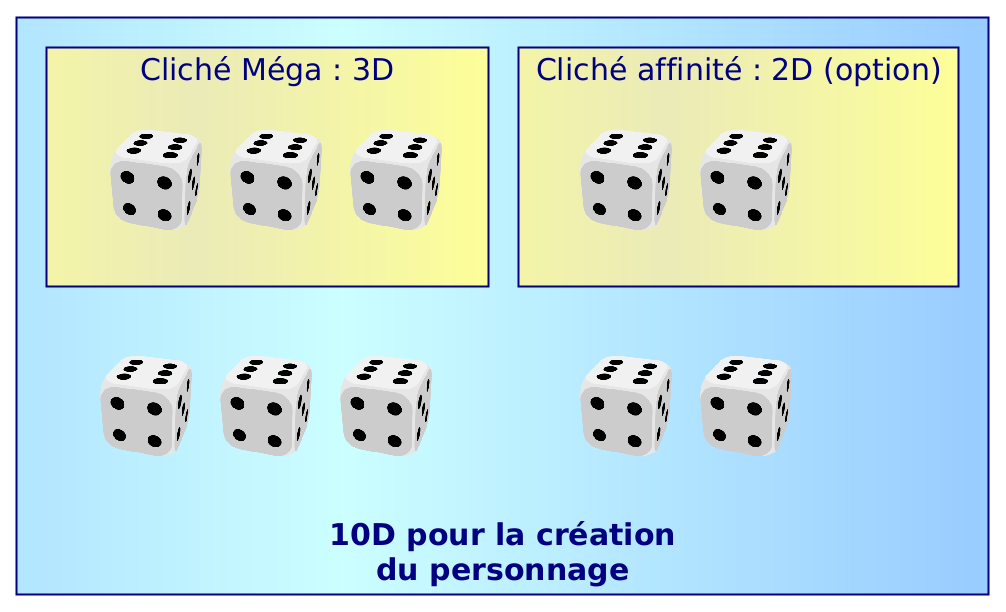
\includegraphics[scale=0.28]{01-creation-perso}
\end{center}

Exemple de Clichés Méga : Terrien Méga des montagnes, Méga parisien impressionné par la grandeur de l'univers, Méga kiffant les mondes parallèles, Méga intello qui veut tout comprendre, Méga hystérique de jouer avec ses pouvoirs, Méga prudent et travailleur, Méga qui a peur de se retrouver sur la Bételgeuse d'un monde parallèle, etc.. 

\subsection{Affinité}

Optionnellement, le Méga peut choisir une affinité (généralement au moins 2D) ou lancer 2D et consulter le diagramme ci-dessous. L'affinité est aussi source de Clichés.

\begin{center}
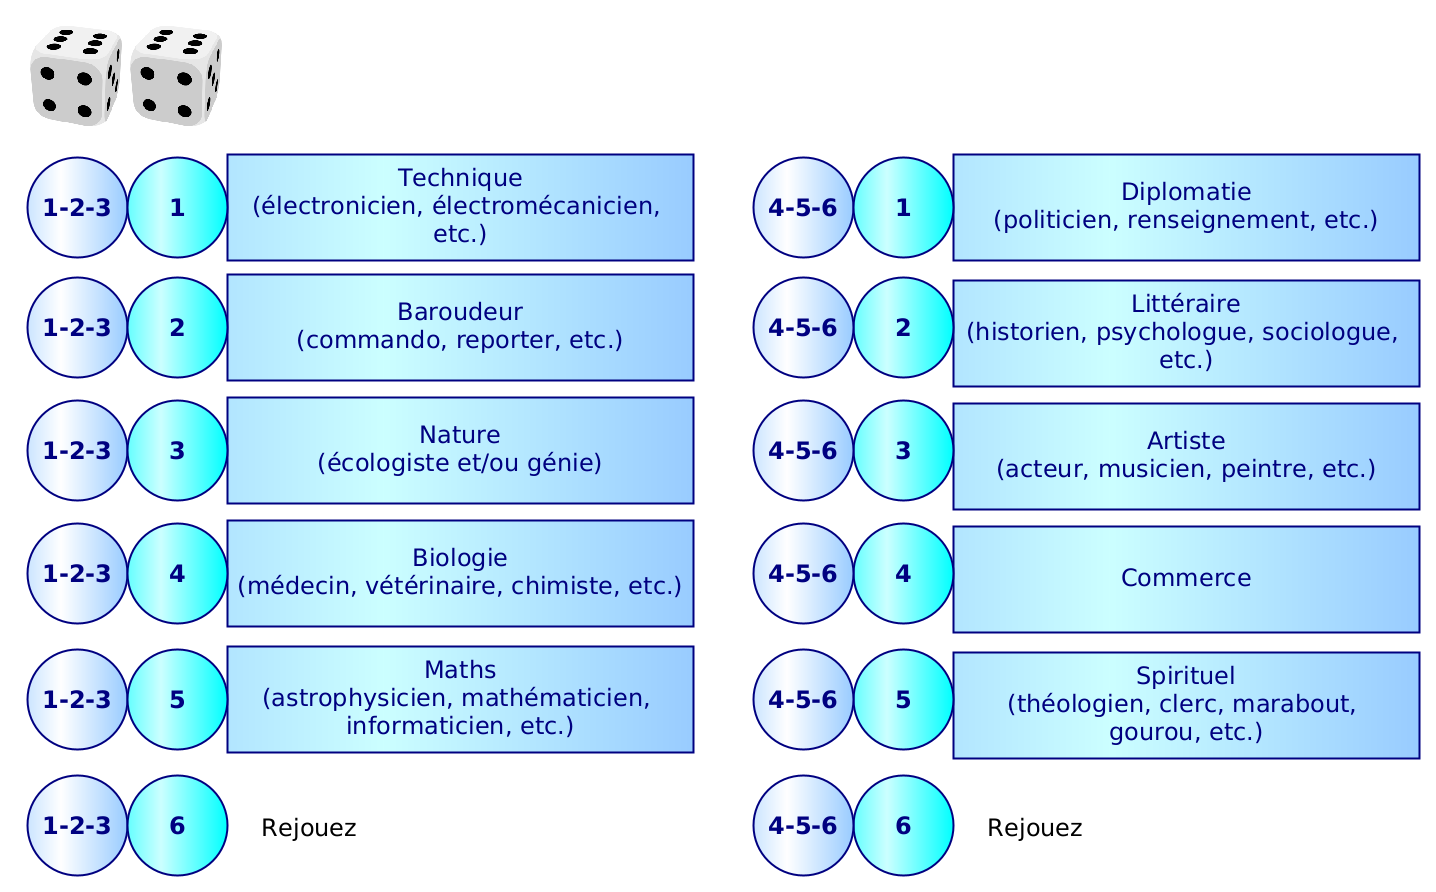
\includegraphics[scale=0.28]{02-affinite}
\end{center}

\newpage
%=================================Nouvelle page
%TODO Pouvoirs psy
\section{Pouvoirs psy}

Les Mégas possèdent déjà deux pouvoirs exceptionnels qui les rendent uniques au sein des univers : le Transit et le Transfert (couverts par le Cliché Méga, voir plus loin).

En supplément, le MJ peut autoriser les Mégas à disposer d'un autre pouvoir psy, soit choisi, soit tiré au sort dans la table ci-dessous.

\begin{center}
\begin{tabular}{c l}

\includegraphics[scale=0.08]{dice.png} & \textbf{Pouvoir psy}\\
1 & Emprunte astrale \\
2 & Télékinésie \\
3 & Télépathie \\
4 & Lévitation \\
5 & Corps éthéral \\
6 & Rejouez \\
\end{tabular}
\end{center}

\begin{center}
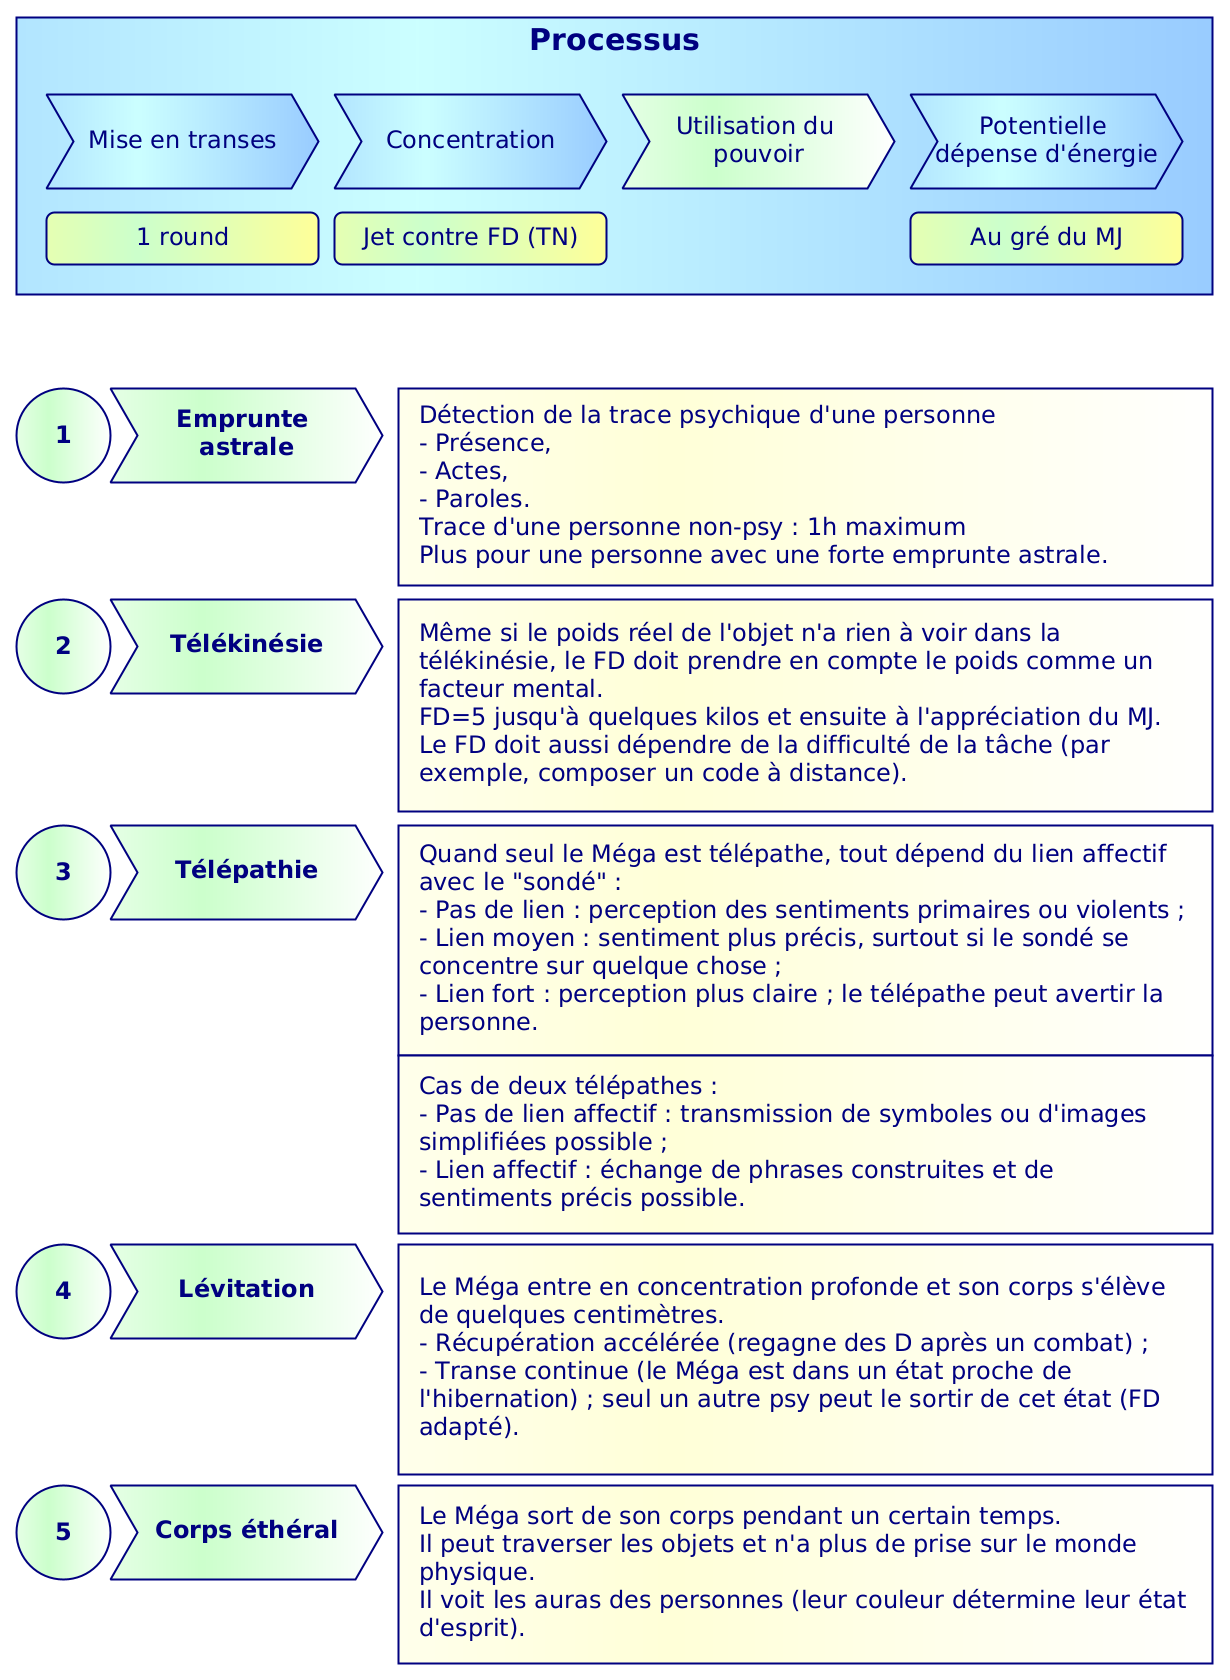
\includegraphics[scale=0.28]{03-pouvoirs-psy}
\end{center}

\newpage
%=================================Nouvelle page
%TODO Le Transit
\section{Le Transit}

\subsection{Règles du Transit}

Le Transit est la faculté de se téléporter au moyen d'un tétraèdre, soit dans le même univers, soit dans un univers parallèle.

Le premier Transit est facile, mais les Transits subséquents sont plus difficiles et coûtent un ou plusieurs dés de Mégas de manière temporaire (au jugé du MJ). Voir les étiquettes pour les facteurs de difficultés (FD) et les pertes de dés.

\begin{center}
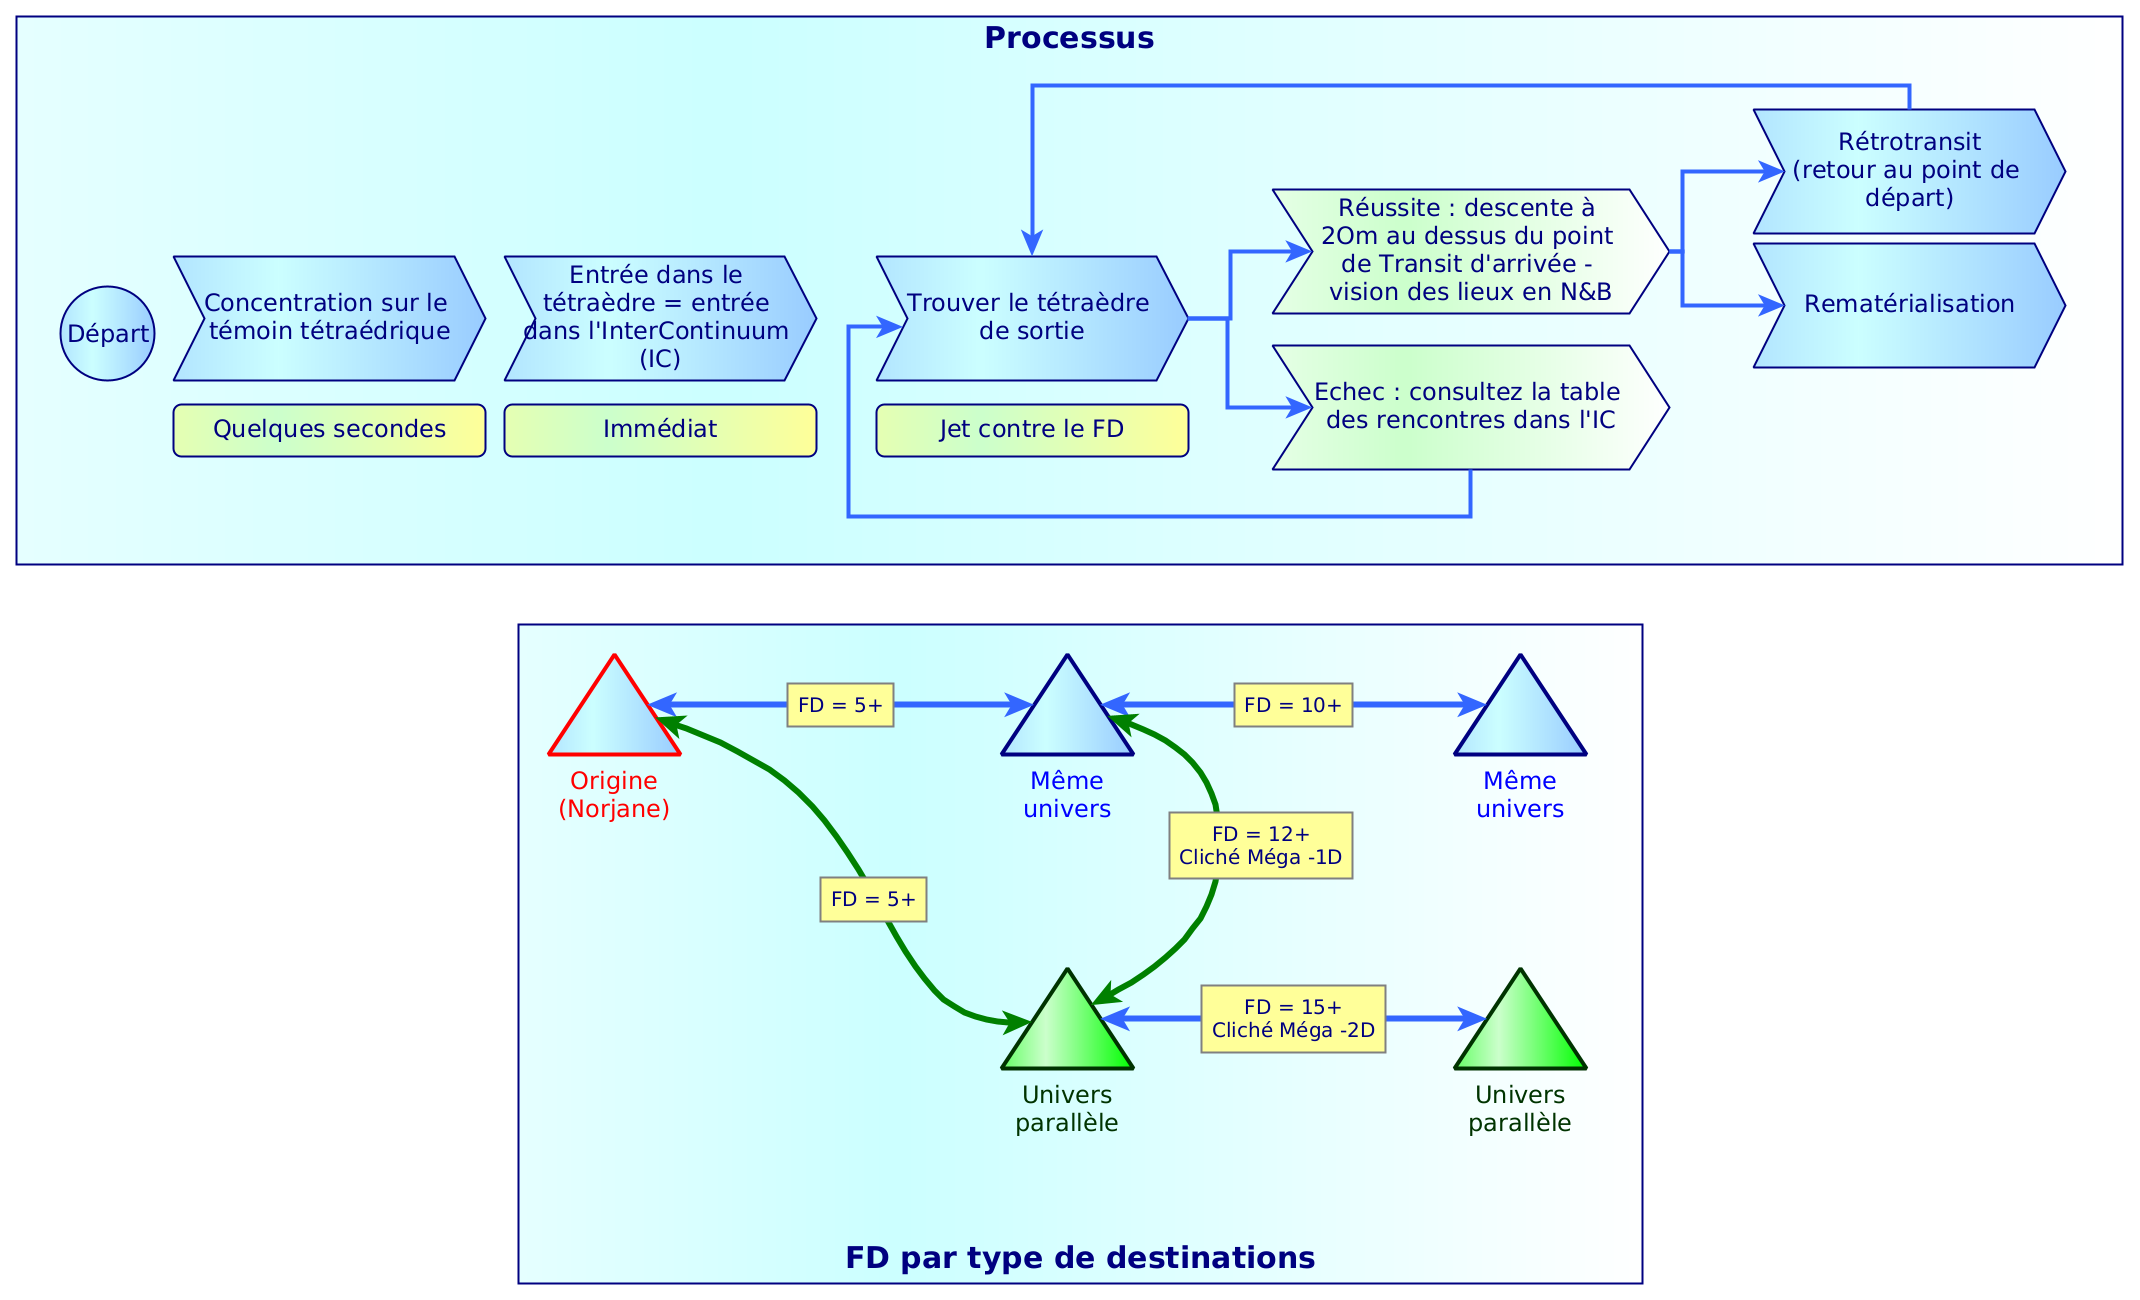
\includegraphics[scale=0.3]{04-transit}
\end{center}

En cas d'échec, tout peut arriver, au gré du MJ. Si un PJ a créé un ou des points de transit, il a 50\% de chances d'aboutir sur un d'entre eux (tirer point après point).

Il est possible de transiter avec un autre être vivant, pourvu que l'on reste en contact avec lui. Le MJ peut ajouter un FD supplémentaire au FD du dessus (entre +3 et +5).

\subsection{Créer un point de Transit}

Le MJ détermine la résistance du point de Transit en lançant 8D ou plus. Par exemple, supposons que la résistance du tétraèdre soit de 27. Le Méga doit accumuler plus de 27 points en faisant des jets contre un FD de 11 et en suivant le processus ci-dessous.


\begin{center}
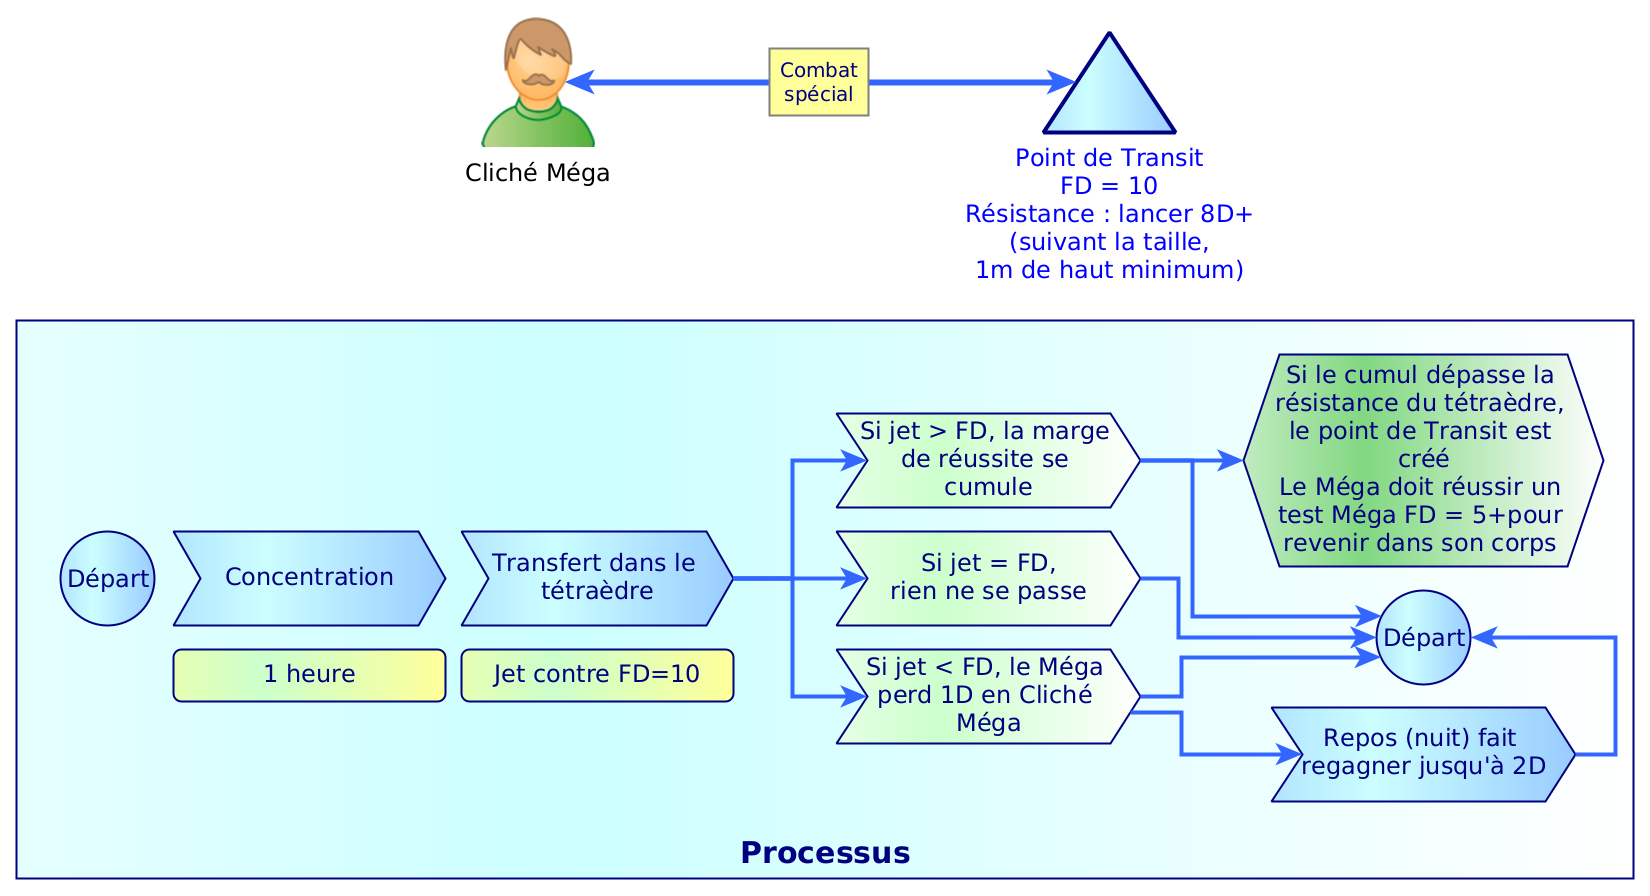
\includegraphics[scale=0.28]{05-point-transit}
\end{center}



\newpage
%=================================Nouvelle page
%TODO Le Transfert
\section{Le Transfert}

Le Transfert est la capacité de se transférer dans le corps d'un autre être vivant.  C'est un combat mental.

En cas de Transfert réussi, le corps du Méga tombe en catalepsie.

La figure ci-dessous montre une interprétation des règles du Transfert pour Risus Méga. Le Transfert est normalement assez facile, mais il a des effets secondaires (rejet de l'hôte). A noter : un transfert depuis un corps transféré est un combat contre la somme des Clichés des hôtes (départ et arrivée).


\begin{center}
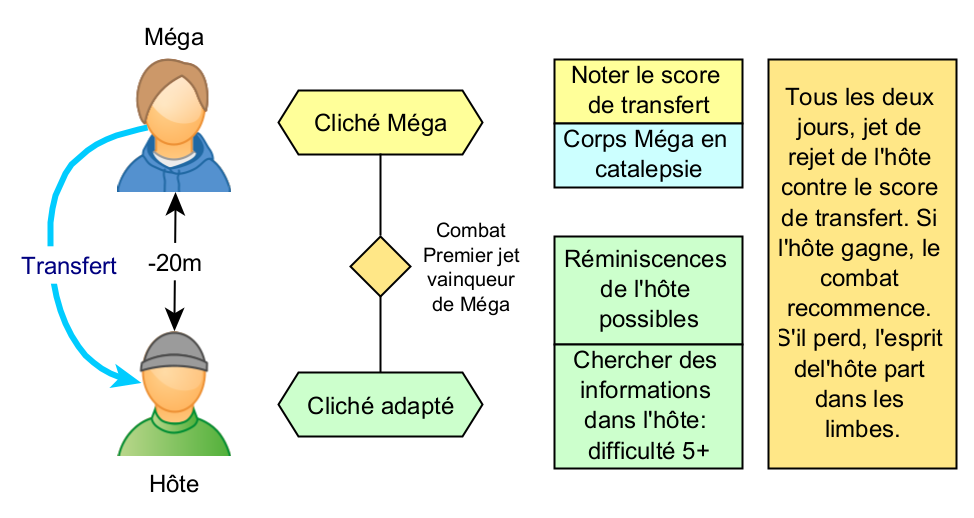
\includegraphics[scale=.4]{mega-transfert}
\end{center}





\end{document}
